\section{The point of complex multiplication in coordinates}\label{app:cmpoint}

This appendix works out, in coordinates, the objects of Lemma~\ref{lem:cmext} and Proposition~\ref{prop:twostep} on $A_{0}=E_{0}^{6}$: the Hodge ring, the Weil plane, an explicit family of abelian threefolds whose classes combine to the Weil class, their intersection numbers, and the dimensions of every Ext group between the pieces built from them.

\begin{table}[t]
\centering
\caption{The Ext groups between two pieces at $A_{0}=E_{0}^{6}$, from Lemma~\ref{lem:cmext}; $m=b-a$, $\chi_{Z}=8$ for the threefolds $Z_{\zeta}$.}
\label{tab:cmext}
\begin{ruledtabular}
\begin{tabular}{llll}
from & to & degrees $k$ & $\dim\Ext^{k}$ \\
\colrule
$\mathcal{O}_{Z}L^{a}$ & $\mathcal{O}_{Z}L^{a}$ & $0,\dots,6$ & $\binom{6}{k}$: $1,6,15,20,15,6,1$ \\
$\mathcal{O}_{Z}L^{a}$ & $\mathcal{O}_{Z}L^{b}$, $m>0$ & $0,\dots,3$ & $\binom{3}{k}\,8m^{3}$ \\
$\mathcal{O}_{Z}L^{a}$ & $\mathcal{O}_{Z}L^{b}$, $m<0$ & $3,\dots,6$ & $\binom{3}{k-3}\,8|m|^{3}$ \\
$\mathcal{O}_{Z}L^{a}$ & $\mathcal{O}_{Z'}L^{b}$ & $3$ & $(Z\cdot Z')\in\{8,16,32,64\}$ \\
$\mathcal{O}_{Z}L^{a}$ & $L^{b}$, $m>0$ & $3$ & $8m^{3}$ \\
$\mathcal{O}_{Z}L^{a}$ & $L^{b}$, $m<0$ & $6$ & $8|m|^{3}$ \\
$\mathcal{O}_{Z}L^{a}$ & $L^{a}$ & $3,\dots,6$ & $\binom{3}{k-3}$ \\
$L^{a}$ & $\mathcal{O}_{Z}L^{b}$, $m>0$ & $0$ & $8m^{3}$ \\
$L^{a}$ & $\mathcal{O}_{Z}L^{b}$, $m<0$ & $3$ & $8|m|^{3}$ \\
$L^{a}$ & $\mathcal{O}_{Z}L^{a}$ & $0,\dots,3$ & $\binom{3}{k}$ \\
$L^{a}$ & $L^{b}$, $m>0$ & $0$ & $m^{6}$ \\
$L^{a}$ & $L^{b}$, $m<0$ & $6$ & $|m|^{6}$ \\
$L^{a}$ & $L^{a}$ & $0,\dots,6$ & $\binom{6}{k}$ \\
\end{tabular}
\end{ruledtabular}
\end{table}

\begin{figure*}[t]
\centering
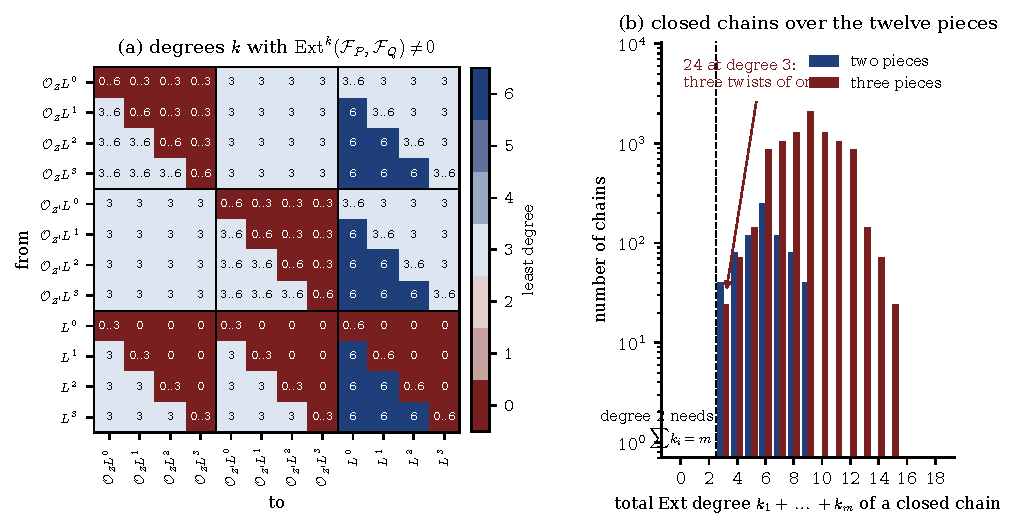
\includegraphics[width=0.96\textwidth]{figures/fig_extgrid}
\caption{The degrees of the Ext groups between the twelve pieces $\mathcal{O}_{Z}L^{k}$, $\mathcal{O}_{Z'}L^{k}$, $L^{k}$, $k=0,\dots,3$, of Table~\ref{tab:cmext}. Left: the degrees in which $\Ext^{k}(\mathcal{F}_{P},\mathcal{F}_{Q})$ is nonzero, coloured by the least one; degree zero occurs only from a lower twist to a higher one and from $L^{a}$ to $\mathcal{O}_{Z}L^{a}$. Right: the number of closed chains of two and of three distinct pieces by total degree, on a logarithmic scale; no two-piece chain has total degree below three, and the three-piece chains of total degree three are those of Proposition~\ref{prop:twostep}.}
\label{fig:extgrid}
\end{figure*}

\begin{figure*}[t]
\centering
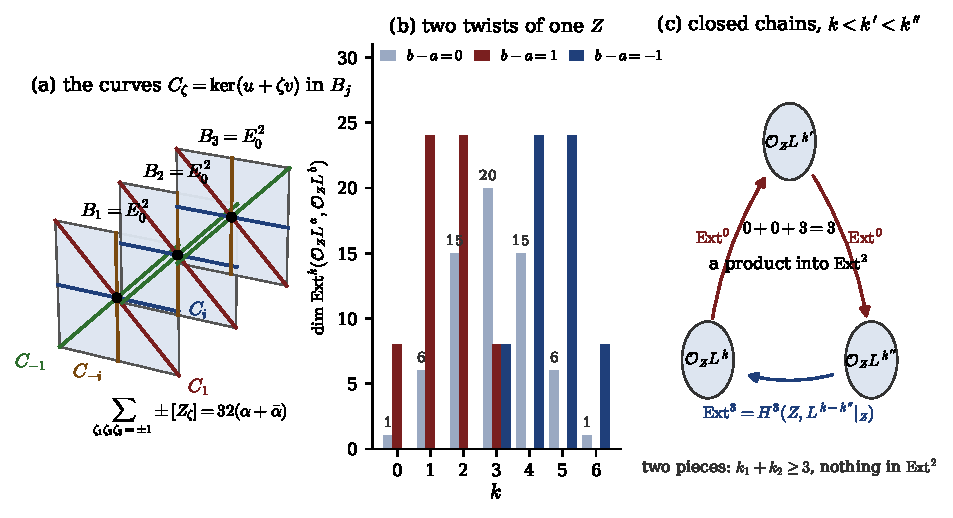
\includegraphics[width=\textwidth]{figures/fig_cmpoint}
\caption{The point $E_{0}^{6}$ of complex multiplication. Left: the three Weil surfaces $B_{j}=E_{0}^{2}$ and the four elliptic curves $C_{\zeta}$ in each, kernels of $u+\zeta v$; a threefold $Z_{\zeta}$ picks one curve in each surface, and the $32$ threefolds with $\zeta_{1}\zeta_{2}\zeta_{3}=\pm1$, signed by that product, add up to $32(\alpha+\bar\alpha)$. Middle: the dimensions of $\Ext^{k}(\mathcal{O}_{Z}\otimes L^{a},\mathcal{O}_{Z}\otimes L^{b})$ by degree for $b-a=0$ (the $\binom{6}{k}$), $b-a=1$ (degrees $0$ to $3$) and $b-a=-1$ (degrees $3$ to $6$). Right: the closed chains of Proposition~\ref{prop:twostep}; every two-step chain has total degree at least three, and the shortest chains reaching degree two run through three twists of one threefold with degrees $0,0,3$.}
\label{fig:cmpoint}
\end{figure*}

\subsection{The forms and the Hodge ring}\label{app:forms}

Write $z_{1},\dots,z_{6}$ for the coordinates of $A_{0}=E_{0}^{6}$, $E_{0}=\CC/\ZZ[i]$, group the factors into the three surfaces $B_{j}=E_{0}^{2}$ with coordinates $(z_{j},z_{3+j})$, $j=1,2,3$, and let $K=\QQ(i)$ act by $i$ on $z_{1},z_{2},z_{3}$ and by $-i$ on $z_{4},z_{5},z_{6}$. Put
\begin{equation}\label{eq:cmforms}
\begin{aligned}
a_{j}&=\tfrac{i}{2}\,dz_{j}\wedge d\bar z_{j}, &
b_{j}&=\tfrac{i}{2}\,dz_{3+j}\wedge d\bar z_{3+j},\\
c_{j}&=\tfrac{i}{2}\,dz_{j}\wedge d\bar z_{3+j}, &
\bar c_{j}&=\tfrac{i}{2}\,dz_{3+j}\wedge d\bar z_{j}.
\end{aligned}
\end{equation}
In the real coordinates $z_{j}=x_{j}+iy_{j}$ one has $a_{j}=dx_{j}\wedge dy_{j}$, the volume form of the $j$-th factor, of integral one over $\CC/\ZZ[i]$,\footnote{The fundamental domain of $\ZZ[i]$ is the unit square, so $\int_{E_{0}}dx\wedge dy=1$; this normalisation makes every form in \eqref{eq:cmforms} integral on the lattice $\ZZ[i]^{6}$, and all intersection numbers below are integers computed as integrals of top forms.} and $c_{j}=\tfrac12(dx_{j}\wedge dy_{3+j}-dy_{j}\wedge dx_{3+j})+\tfrac{i}{2}(dx_{j}\wedge dx_{3+j}+dy_{j}\wedge dy_{3+j})$, so that the real and imaginary parts of $c_{j}$ are rational classes and $\bar c_{j}$ is the complex conjugate of $c_{j}$. All four forms have type $(1,1)$. The polarisation is
\begin{equation}\label{eq:cmtheta}
\theta=\sum_{j=1}^{3}(a_{j}+b_{j}),\qquad \theta^{6}=6!\,a_{1}b_{1}a_{2}b_{2}a_{3}b_{3},\qquad \int_{A_{0}}\frac{\theta^{6}}{6!}=1,
\end{equation}
the principal polarisation of the product; the hermitian forms $\sum_{j\le3}a'_{j}z_{j}\bar w_{j}-\sum_{j>3}a'_{j}z_{j}\bar w_{j}$ of Lemma~\ref{lem:cmext} with all $a'_{j}=1$ give $\theta$ itself.

The Hodge group of $A_{0}$ is the circle acting by $z$ on $H^{1,0}$ and by $\bar z$ on $H^{0,1}$, so the Hodge classes of degree $2k$ are exactly the rational classes of type $(k,k)$, of dimension $\binom{6}{k}^{2}$:
\begin{equation}\label{eq:cmdims}
\dim\Hdg^{2k}(A_{0})=1,\,36,\,225,\,400,\,225,\,36,\,1\quad(k=0,\dots,6).
\end{equation}
In degree two these are the $36$ hermitian forms on $\ZZ[i]^{6}$, the Picard number of $E_{0}^{6}$. The $K$-eigenspaces of $H^{1}(A_{0},\CC)$ are spanned by $dz_{1},dz_{2},dz_{3},d\bar z_{4},d\bar z_{5},d\bar z_{6}$ (eigenvalue $i$) and by their conjugates, so the Weil plane $W=\bigwedge^{6}_{K}H^{1}(A_{0},K)\subseteq H^{6}(A_{0},\QQ)$ is spanned over $\CC$ by
\begin{equation}\label{eq:cmweil}
\alpha=c_{1}c_{2}c_{3}\propto dz_{1}dz_{2}dz_{3}\,d\bar z_{4}d\bar z_{5}d\bar z_{6}\qquad\text{and}\qquad\bar\alpha=\bar c_{1}\bar c_{2}\bar c_{3},
\end{equation}
and over $\QQ$ by $\alpha+\bar\alpha$ and $i(\alpha-\bar\alpha)$. The relation $W\theta=0$ is visible term by term: $c_{j}a_{j}$ contains $dz_{j}$ twice and $c_{j}b_{j}$ contains $d\bar z_{3+j}$ twice, so $\alpha\,(a_{k}+b_{k})=0$ for each $k$, since $\alpha$ already contains $dz_{k}$ and $d\bar z_{3+k}$.

\subsection{The elliptic curves \texorpdfstring{$C_{\zeta}$}{C} and the threefolds \texorpdfstring{$Z_{\zeta}$}{Z}}\label{app:curves}

For $\zeta\in\mu_{4}=\{1,i,-1,-i\}$ let $C_{\zeta}\subseteq B_{j}$ be the kernel of $(u,v)\mapsto u+\zeta v$, an elliptic curve isomorphic to $E_{0}$, and for $\zeta=(\zeta_{1},\zeta_{2},\zeta_{3})\in\mu_{4}^{3}$ let $Z_{\zeta}=C_{\zeta_{1}}\times C_{\zeta_{2}}\times C_{\zeta_{3}}\subseteq A_{0}$, an abelian threefold.

\begin{lemma}\label{lem:cmcurves}
\begin{enumerate}[label=\textup{(\roman*)},leftmargin=2.4em,itemsep=2pt]
\item $[C_{\zeta}]=a_{j}+b_{j}+\bar\zeta\,c_{j}+\zeta\,\bar c_{j}$ in $H^{2}(B_{j})$, and $[Z_{\zeta}]=\prod_{j}[C_{\zeta_{j}}]$.
\item $(C_{\zeta}\cdot C_{\zeta'})=|\zeta-\zeta'|^{2}\in\{0,2,4\}$ on $B_{j}$; $Z_{\zeta}\cap Z_{\zeta'}$ is finite exactly when $\zeta_{j}\ne\zeta'_{j}$ for all $j$, and then $|Z_{\zeta}\cap Z_{\zeta'}|=\prod_{j}|\zeta_{j}-\zeta'_{j}|^{2}\in\{8,16,32,64\}$.
\item $\theta|_{Z_{\zeta}}$ has degree two on each factor, $(\theta|_{Z_{\zeta}})^{3}=48$ and $\chi_{Z_{\zeta}}=8$; in particular $[Z_{\zeta}]\theta\ne0$.
\item Writing $S(\omega)=\sum_{\zeta_{1}\zeta_{2}\zeta_{3}=\omega}[Z_{\zeta}]$ for $\omega\in\mu_{4}$,
\begin{equation}\label{eq:cmgenerating}
\begin{gathered}
\sum_{\omega\in\mu_{4}}\omega^{m}S(\omega)=\prod_{j=1}^{3}T_{m,j},\qquad T_{m,j}=\sum_{\zeta\in\mu_{4}}\zeta^{m}[C_{\zeta}],\\
T_{m,j}=4(a_{j}+b_{j}),\ 4c_{j},\ 0,\ 4\bar c_{j}\quad\text{for }m\equiv0,1,2,3\pmod 4,
\end{gathered}
\end{equation}
and therefore
\begin{equation}\label{eq:cm32}
S(1)-S(-1)=\sum_{\zeta_{1}\zeta_{2}\zeta_{3}=1}[Z_{\zeta}]-\sum_{\zeta_{1}\zeta_{2}\zeta_{3}=-1}[Z_{\zeta}]=32\,(\alpha+\bar\alpha).
\end{equation}
\end{enumerate}
\end{lemma}

\begin{proof}
(i) $C_{\zeta}$ is the fibre over $0$ of the surjective homomorphism $f_{\zeta}\colon B_{j}\to E_{0}$, $w=u+\zeta v$, so $[C_{\zeta}]=f_{\zeta}^{*}[0]$ with $[0]=\tfrac{i}{2}dw\wedge d\bar w$, and
\begin{align*}
dw\wedge d\bar w&=(du+\zeta\,dv)\wedge(d\bar u+\bar\zeta\,d\bar v)\\
&=du\wedge d\bar u+dv\wedge d\bar v+\bar\zeta\,du\wedge d\bar v+\zeta\,dv\wedge d\bar u ,
\end{align*}
which is the formula. A product of subvarieties of the factors has the product class.

(ii) On $B_{j}$ the only nonzero products of two of the four forms are $a_{j}b_{j}$ and $c_{j}\bar c_{j}=\bar c_{j}c_{j}=-a_{j}b_{j}$ (reorder $du\,d\bar v\,dv\,d\bar u$ to $-du\,d\bar u\,dv\,d\bar v$), and $\int_{B_{j}}a_{j}b_{j}=1$. Hence $[C_{\zeta}][C_{\zeta'}]=2-\bar\zeta\zeta'-\zeta\bar\zeta'=|\zeta-\zeta'|^{2}$. Directly: a point of $C_{\zeta}\cap C_{\zeta'}$ has $(\zeta-\zeta')v=0$, so $v$ runs over the kernel of $\zeta-\zeta'$ on $E_{0}$, of order $|\zeta-\zeta'|^{2}$, and $u=-\zeta v$ is then determined. The statement for $Z_{\zeta}$ follows factor by factor.

(iii) $\int_{C_{\zeta}}(a_{j}+b_{j})=\int_{B_{j}}(a_{j}+b_{j})[C_{\zeta}]=2$, since $a_{j}c_{j}$, $a_{j}\bar c_{j}$, $b_{j}c_{j}$, $b_{j}\bar c_{j}$ all repeat a differential. So $\theta|_{Z_{\zeta}}=2(p_{1}+p_{2}+p_{3})$ with $p_{j}$ the point class of the $j$-th factor, $(\theta|_{Z_{\zeta}})^{3}=3!\cdot8=48$, and $\chi_{Z_{\zeta}}=48/6=8$.

(iv) The left side of \eqref{eq:cmgenerating} is $\sum_{\zeta}(\zeta_{1}\zeta_{2}\zeta_{3})^{m}\prod_{j}[C_{\zeta_{j}}]$, which factors as the product of the three sums $T_{m,j}$; these are read off from (i), using $\sum_{\zeta\in\mu_{4}}\zeta^{m}=4$ or $0$ according as $4\mid m$ or not. Then $S(1)-S(-1)=\tfrac12\sum_{\omega}(\omega+\omega^{3})S(\omega)=\tfrac12\bigl(\prod_{j}T_{1,j}+\prod_{j}T_{3,j}\bigr)=\tfrac12(64\alpha+64\bar\alpha)$.
\end{proof}

Equation \eqref{eq:cm32} is the analogue, with abelian threefolds in place of line bundles, of the signed sum of the $32$ line bundles on $E_{0}^{6}$ in \cite[Prop.~18.21]{BMB26}: the $32$ threefolds $Z_{\zeta}$ with $\zeta_{1}\zeta_{2}\zeta_{3}=\pm1$, taken with the sign $\zeta_{1}\zeta_{2}\zeta_{3}$, have classes adding up to $32$ times the real Weil class. Together with three powers of $L$ this is a Chern character of polarised shape and Hankel rank three at $A_{0}$, and by Lemma~\ref{lem:cmext}(i) it is one of the shapes a convolution must realise. Two of these threefolds with $\zeta_{j}=\zeta'_{j}$ for one or two indices $j$ meet along a curve or a surface, so Lemma~\ref{lem:cmext}(ii) does not apply to them and Lemma~\ref{lem:cmmeet} gives their groups; Proposition~\ref{prop:separated} shows that no convolution of these thirty-five pieces meets the criterion. Figure~\ref{fig:cmpoint} draws the curves, the dimensions of the Ext groups and the chains.

\subsection{The dimensions in Lemma~\ref{lem:cmext}}\label{app:extdims}

For the threefolds $Z=Z_{\zeta}$ the numbers of Lemma~\ref{lem:cmext} are explicit. Table~\ref{tab:cmext} lists, for every pair of piece types, the degrees $k$ in which $\Ext^{k}$ is nonzero and its dimension; here $m=b-a$ is the difference of the twists, $\chi_{Z}=8$, $Z'=Z_{\zeta'}$ with $\zeta_{j}\ne\zeta'_{j}$ for all $j$, and $(Z\cdot Z')=\prod_{j}|\zeta_{j}-\zeta'_{j}|^{2}$.



Each row of the table restates the corresponding item of Lemma~\ref{lem:cmext}, with $\chi(L^{m}|_{Z})=m^{3}\chi_{Z}=8m^{3}$ from (iii) above and $\chi(L^{m})=m^{6}\theta^{6}/720=m^{6}$ from \eqref{eq:cmtheta}. Two features of the table drive Proposition~\ref{prop:twostep}. Every group between two pieces of different twist is concentrated in degree $0$, in degree $3$ or $6$, or in the range $0$ to $3$ for two twists of one threefold; and a group in degree at most two between distinct pieces occurs only from a lower twist to a higher one, or from $L^{a}$ to $\mathcal{O}_{Z}L^{a}$. The bookkeeping of the proposition is then the following count. A closed chain of $m$ pieces whose edges have Ext degrees $k_{1},\dots,k_{m}$ carries an $m$-fold product into $\Ext^{\sum k_{i}-m+2}$ of the first piece. For $m=2$ the table gives, for each unordered pair of distinct piece types, the two degrees and their sum:
\begin{equation}\label{eq:cmtwostep}
\begin{array}{lll}
(\mathcal{O}_{Z}L^{a},\mathcal{O}_{Z'}L^{b}) & 3+3 & =6,\\
(\mathcal{O}_{Z}L^{a},\mathcal{O}_{Z}L^{b}),\ b>a & (0\text{ to }3)+(3\text{ to }6) & \ge3,\\
(\mathcal{O}_{Z}L^{a},L^{b}),\ b>a & 3+3 & =6,\\
(\mathcal{O}_{Z}L^{a},L^{b}),\ b<a & 6+0 & =6,\\
(\mathcal{O}_{Z}L^{a},L^{a}) & (3\text{ to }6)+(0\text{ to }3) & \ge3,\\
(L^{a},L^{b}) & 0+6 & =6,
\end{array}
\end{equation}
so no two-step product reaches degree two. For $m=3$ the sum must be $3$ with two edges of degree zero, and the table leaves exactly the ascending chains $\mathcal{O}_{Z}L^{k}\to\mathcal{O}_{Z}L^{k'}\to\mathcal{O}_{Z}L^{k''}$, $k<k'<k''$, closed by the degree-three edge $H^{3}(Z,L^{k-k''}|_{Z})$, of dimension $8(k''-k)^{3}$. The program \path{code/cm_point_ext.py} enumerates the chains of two and three pieces over four twists and two threefolds and confirms both statements, together with the identities of Lemma~\ref{lem:cmcurves}. Figure~\ref{fig:extgrid} shows the table as the matrix of the twelve pieces, and the distribution of the total degree over every closed chain of two and of three distinct pieces: the two-piece chains begin at total degree three, and the twenty-four ordered three-piece chains of total degree three are the eight ascending triples of twists of one threefold, each read from its three starting pieces.


